\documentclass[]{article}
\usepackage{lmodern}
\usepackage{amssymb,amsmath}
\usepackage{ifxetex,ifluatex}
\usepackage{fixltx2e} % provides \textsubscript
\ifnum 0\ifxetex 1\fi\ifluatex 1\fi=0 % if pdftex
  \usepackage[T1]{fontenc}
  \usepackage[utf8]{inputenc}
\else % if luatex or xelatex
  \ifxetex
    \usepackage{mathspec}
  \else
    \usepackage{fontspec}
  \fi
  \defaultfontfeatures{Ligatures=TeX,Scale=MatchLowercase}
\fi
% use upquote if available, for straight quotes in verbatim environments
\IfFileExists{upquote.sty}{\usepackage{upquote}}{}
% use microtype if available
\IfFileExists{microtype.sty}{%
\usepackage{microtype}
\UseMicrotypeSet[protrusion]{basicmath} % disable protrusion for tt fonts
}{}
\usepackage[margin=1in]{geometry}
\usepackage{hyperref}
\hypersetup{unicode=true,
            pdftitle={PrEP and Porn: Trends in Popularity of Condom-less Pornographic Videos featuring Men having Sex with Men},
            pdfauthor={Kenneth Morales},
            pdfborder={0 0 0},
            breaklinks=true}
\urlstyle{same}  % don't use monospace font for urls
\usepackage{graphicx,grffile}
\makeatletter
\def\maxwidth{\ifdim\Gin@nat@width>\linewidth\linewidth\else\Gin@nat@width\fi}
\def\maxheight{\ifdim\Gin@nat@height>\textheight\textheight\else\Gin@nat@height\fi}
\makeatother
% Scale images if necessary, so that they will not overflow the page
% margins by default, and it is still possible to overwrite the defaults
% using explicit options in \includegraphics[width, height, ...]{}
\setkeys{Gin}{width=\maxwidth,height=\maxheight,keepaspectratio}
\IfFileExists{parskip.sty}{%
\usepackage{parskip}
}{% else
\setlength{\parindent}{0pt}
\setlength{\parskip}{6pt plus 2pt minus 1pt}
}
\setlength{\emergencystretch}{3em}  % prevent overfull lines
\providecommand{\tightlist}{%
  \setlength{\itemsep}{0pt}\setlength{\parskip}{0pt}}
\setcounter{secnumdepth}{0}
% Redefines (sub)paragraphs to behave more like sections
\ifx\paragraph\undefined\else
\let\oldparagraph\paragraph
\renewcommand{\paragraph}[1]{\oldparagraph{#1}\mbox{}}
\fi
\ifx\subparagraph\undefined\else
\let\oldsubparagraph\subparagraph
\renewcommand{\subparagraph}[1]{\oldsubparagraph{#1}\mbox{}}
\fi

%%% Use protect on footnotes to avoid problems with footnotes in titles
\let\rmarkdownfootnote\footnote%
\def\footnote{\protect\rmarkdownfootnote}

%%% Change title format to be more compact
\usepackage{titling}

% Create subtitle command for use in maketitle
\newcommand{\subtitle}[1]{
  \posttitle{
    \begin{center}\large#1\end{center}
    }
}

\setlength{\droptitle}{-2em}
  \title{PrEP and Porn: Trends in Popularity of Condom-less Pornographic Videos
featuring Men having Sex with Men}
  \pretitle{\vspace{\droptitle}\centering\huge}
  \posttitle{\par}
  \author{Kenneth Morales}
  \preauthor{\centering\large\emph}
  \postauthor{\par}
  \predate{\centering\large\emph}
  \postdate{\par}
  \date{October 22, 2017}

\usepackage{booktabs}
\usepackage{longtable}
\usepackage{array}
\usepackage{multirow}
\usepackage[table]{xcolor}
\usepackage{wrapfig}
\usepackage{float}
\usepackage{colortbl}
\usepackage{pdflscape}
\usepackage{tabu}
\usepackage{threeparttable}
\usepackage{amssymb, amsmath, booktabs, multirow}

\begin{document}
\maketitle

{
\setcounter{tocdepth}{2}
\tableofcontents
}
\subsubsection{Introduction}\label{introduction}

The film scholar Linda Williams has compared different kinds of
pornography, revealing what she termed a proliferation of ``diff'rent
strokes for diff'rent folks.'' Since sexually explicit media (SEM) first
came into its own in the 1970s with the beginnings of a mainstream
pornographic film industry, diversification of imagery has been a
central ongoing aspect of modern pornography. Since its inception, the
internet has opened up niches for producers and broadcasters targeting a
wide range of specific sexual desires (Williams, 1992). In Williams'
early article, sadomasochistic, homosexual, and bisexual pornographies
are taken to illustrate a gap between then norm and ``perversity,''
without taking into account the new interactions between categories that
stem from their co-existence. In the age of PageRank and the growing
corporate dominance of pornographic production studios, however, the
tyranny of the masses in SEM exemplifies a counter current: the
proliferation of pornographic categories can show how hegemonic desires
provide a path to other desires still, but also how other desires can be
subsumed in hegemonic ones.

Barebacking, or penetrative anal sex without a condom between two men,
could be a rising hegemonic desire in gay pornography. SEM has a variety
of genres; some SEM portray sexual behaviors that range from `vanilla'
(i.e., kissing, oral sex, vaginal sex, anal sex) to `kink' (i.e.,
extreme penetration, water sports, sadomasochism). Safer sex practices,
including the portrayal of condom use, is also highly variable in SEM.
Studios that primarily feature men having sex with men have generally
upheld a self-imposed standard of condom use in anal sex as a response
to the AIDS crisis (Grudzen 2009). Concerns for the health of performers
and the effects of SEM viewership on consumer sex practices have led to
policies like California's Measure B, which mandates the use of condoms
in SEM (Los Angeles Times, 2012).

While condom-less gay porn existed, it was commonly regarded as kink,
and was the domain of specialized or heterodox smaller production
studios. In recent years, however, porn studios have begun dropping the
condom use standard, in response to competition from ``tube'' sites
(such as PornHub), which aggregate and disseminate pornography, and
burgeoning competition from amateur pornographers, many of whom provide
bareback porn unrestrained by mainstream conventions. With the advent of
pre-exposure prophylaxis (PrEP), however, gay porn studios had an out:
they could provide bareback sex for audiences who preferred it while
still bearing the mantle of ``safer'' sex.

PrEP is currently used almost exclusively as shorthand for the use of
the antiretroviral drug Truvada, a two-drug combo manufactured by Gilead
Sciences, to prevent the replication of HIV in unexposed populations.
The CDC approved Truvada as PrEP in May of 2014 (CDC, 2014), and most
large gay pornographic studios began producing bareback porn in the
years following the CDC's endorsement.

Since 2011, five studies have examined the effects of gay SEM, all
studying the relationship between bareback SEM consumption and HIV/STI
risk, all of which have demonstrated varying degrees of positive
association between watching unprotected anal intercourse and
participating in the activity in their sex lives (Eaton et al., 2012;
Nelson et al., 2014; Rosser et al., 2013; Stein et al., 2012; Traeen et
al., 2014). Positive effects of SEM consumption among men who have sex
with men (MSM) include sexuality education, particularly among young
MSM, many of whom report learning about sexuality through this medium
(Kubicek, 2010). SEM consumption has been found to positively predict
higher numbers of sex partners (Braun-Courville \& Rojas, 2009), though
other studies did not find the same association (Rosser et al., 2013).

Given the research at present on the effects of bareback pornography on
viewers, the degree of primacy of SEM depicting unprotected anal
intercourse in online pornographic websites is of public health
interest. The purpose of this study is to examine whether there is a
correlation between the condom utilization practices employed in gay
porn videos and their consumers' viewing habits on a major pornographic
website in the last decade and the new guidelines recommended for
Truvada to be used as pre-exposure prophylaxis (PrEP) on May 14, 2014.

\subsubsection{Methods}\label{methods}

I explored the popularity of pornographic videos containing MSM by their
total view count among a cross-sectional sample of SEM videos from a
popular pornographic video site. \href{www.pornhub.com}{PornHub} is the
world's largest pornography website, operating now for 10 years. At the
time of writing, it is the 36th most popular site on the web (Alexa,
2017). PornHub claims itself as a ``platform'' and a ``video host:'' in
such a way, PornHub is capable of reaping the benefits of the massive
traffic generated to its site while claiming no responsibility for the
videos therein. In 2010, the start-up was bought out by a large adult
entertainment conglomerate Manwin (now known as MindGeek), which owns
several other similar ``tube'' sites as well as pornographic video
production studios (Wallace, 2011).

PornHub organizes video files by ``categories'' to differentiate between
types of content. The larger level domain (www.pornhub.com) contains
content most watched by the presumed heterosexual male viewer (men and
women having sex with women), while the subdomain for gay content
(www.pornhub.com/gayporn) contains SEM most watched by the presumed
homosexual male viewer. Videos are separated from these higher level
domains by virtue of being categorized as ``Gay'' or not in the
website's category system.

In order to be eligible for inclusion in the analysis, videos had to
have been present on PornHub's servers at the time of web scraping (from
September 29 - September 30, 2017), be categorized as ``Gay,'' and be
among the 500 videos listed in one of the 39 subcategory site index
listings (N = 10,693, after removal of duplicates). Selection into the
site index listing by category is determined by PornHub's ``recently
featured'' tag on videos. Videos that, by virtue of categorization into
the ``Solo Male'' category, could not have demonstrated the activity of
interest were removed from the sample (1,340 videos). Only one video was
scraped with an upload year prior to 2010, and was dropped from the
analysis, leaving a final total of 9,353. Analyses were performed in R
and videos were scraped with the R package ``rvest'' (R Core Team, 2017;
Wickham, 2016).

Quantile regression and the quantile regression process was applied for
the impact of predictor variables across quantiles. Standard errors were
determined using the Hall-Sheather bandwidth rule and the Frisch-Newton
algorithm was applied to the basic fitting routine due to considerations
of the sample size--both are options available through the ``qreg''
package in R (Koenker, 2017).

The basic model for analyzing the SEM data presumes that the
log-transformed penalized total view count has a linear splined
conditional quantile functions of the form

\[Q_{log(y)} \left ( \tau |x \right )= \left\{\begin{matrix}
\beta _{0} + \beta _{1}x, & x \in \left [0,4.5  \right ]\\ 
\beta _{0} + \beta _{1}x + \beta _{2}x, & x \in \left [4.5,7  \right ]
\end{matrix}\right.\]

for \(\tau \in \left [0,1 \right ]\). Variables of interest were each
video's view count and the year in which the video was uploaded.
Separate analyses were conducted among videos identified as containing
and not containing bareback sex by bareback categorization. Videos
associated with one of these category labels, ``bareback,'' were assumed
to have the activity of interest: condom-less penetrative anal sex
between at least two men. View count, the response variable \(y\), stood
in as a proxy for overall video popularity, and was measured by total
video views at time of scraping. Video upload dates binned by year,
\(x\), were assumed to have been uploaded on Jan 1 of each year. Having
no data on a time series for view count accumulation for each video, all
videos were assumed to have a constant linear rate of growth from 0
views at baseline to their view count when scraped. Total view counts
were then divided by the total amount of time from presumed upload dates
to time of scraping, \(p\), to get an accumulated views estimate one
year after upload. This was done in order to control for a detection
bias that could privilege older videos, which would have had a longer
time to amass views. These values were then log transformed, and the
resultant values were approximately normal by graphical assessment of a
normal quantile-quantile plot and kernel density estimator. Sample size
was too large to use the Shapiro-Wilk test for normality on view count
data. Upload year was rescaled to begin at earliest upload year, 2010 to
ease in interpretation. The term was splined at a presumed knot of 4.5
years after first sample upload, roughly corresponding to the CDC
endorsement of Truvada as PrEP--a dummy variable indicating this
assignment was utilized via interaction to determine the effect of a
potential change in slope coefficient after the proposed cutoff. Data on
all three variables, upload year, total view count, and bareback
categorization) were available for the entire sample.

\subsubsection{Results}\label{results}

Overall counts of videos in the data, binned by upload year and bareback
categorization is presented in Figure 1, along with the top five video
categories by total view count across the sample.

\begin{figure}
\centering
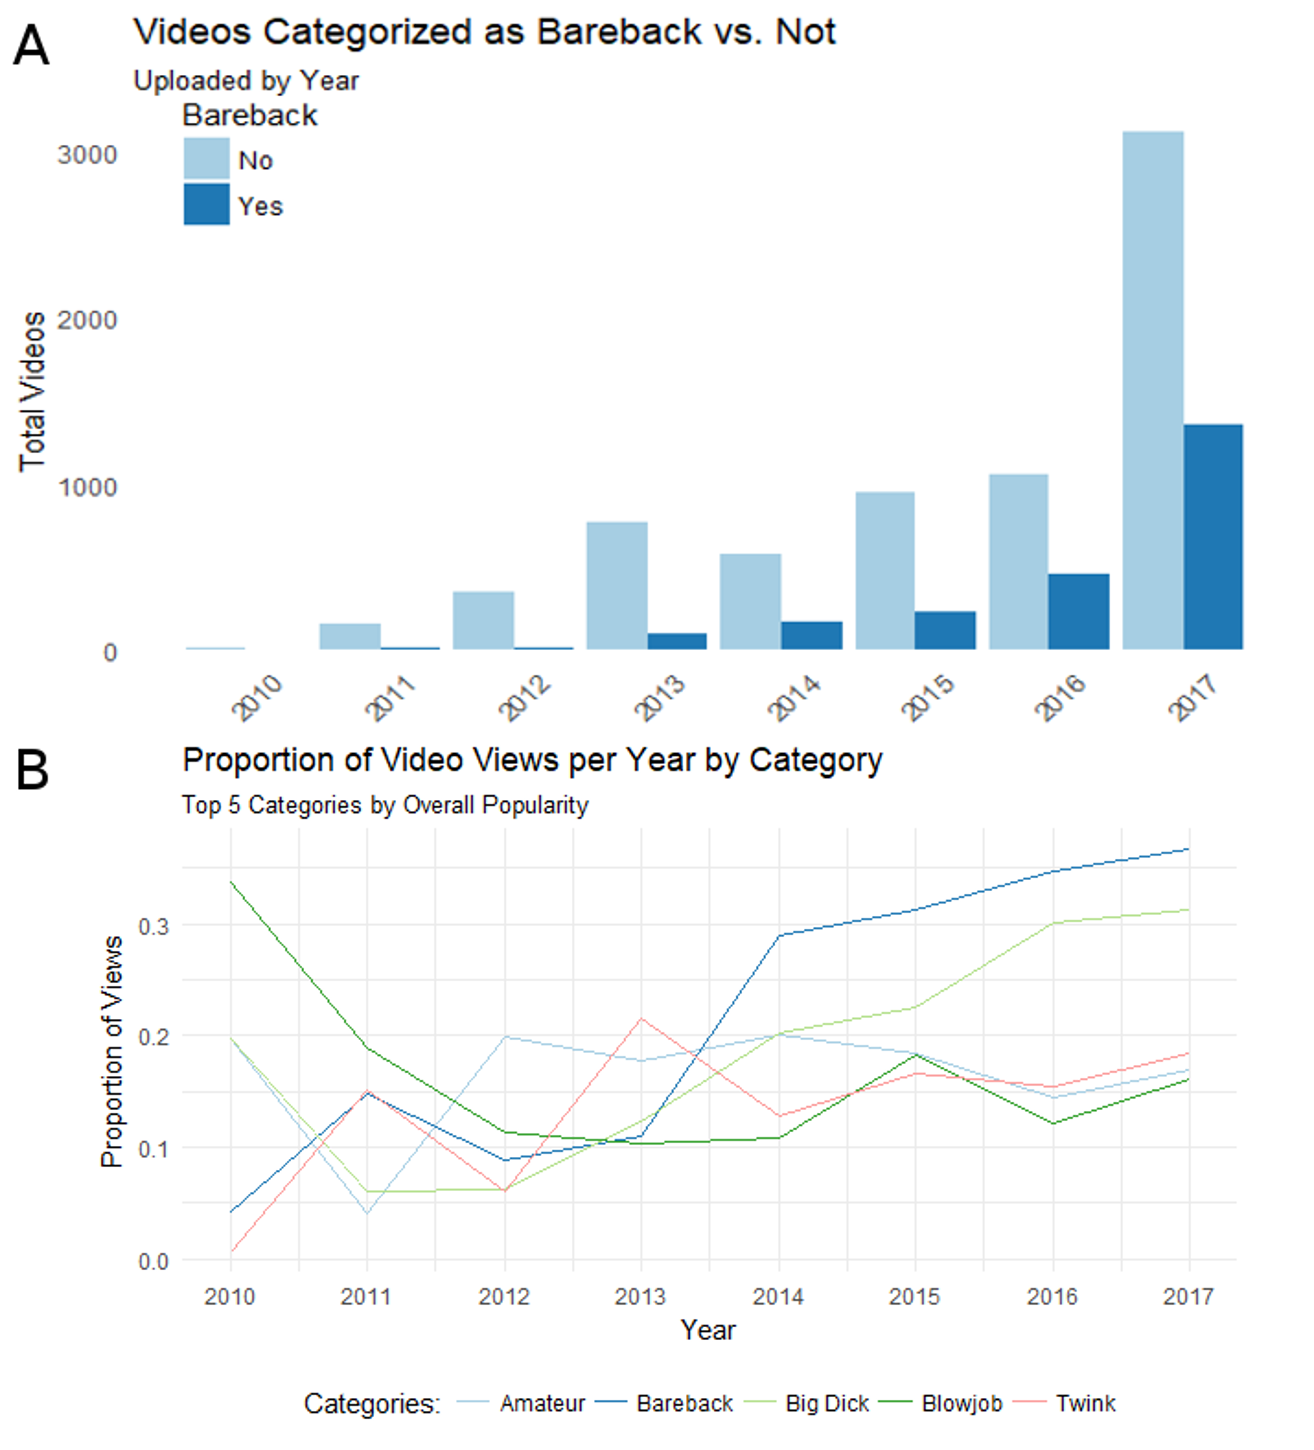
\includegraphics{./bbbyyear.png}
\caption{\emph{Trends in Video Upload Proportions by Bareback
Categorization Across Sample.} A. Upload year was strongly left-skewed.
Proportionally, bareback categorized videos began seeing a marked
increase in upload rates beginning in 2014. These relative subsample
sizes presented graphically here should be kept in mind when discussing
the insights from the quantile regression. B. Across the entire sample,
the five categories with the most views were examined temporally.
Bareback ends up on top at 2017, with over 37\% of all views in that
year attributed to this category of videos. In this sample, the relative
popularity of bareback has increased over time and dominates total
views.}
\end{figure}

Video upload year from the scraped data was strongly left-skewed
(skewness = -1.08) and slightly leptokurtic (kertosis = 3.1). Due to
this skewness and the binned nature of the upload year variable,
quantile regression should serve as a robust method for identifying the
effects on the quantile yearly view counts and interpretations of the
quantile process should not be overly affected by bin size. A strong
recency bias exists in the sample. Assuming the sample is a reasonable
representation of the total upload population on PornHub by upload year,
there is a general trend in a proportional increase in the number of
bareback categorized videos by upload year relative to non-bareback
videos: beginning in 2014, at least a quarter of all videos uploaded in
a given year are bareback, and that proportion gets over 1/3 for the two
most recent years 2016 and 2017. A similar trend is observed by total
views accumulated across the upload years and the five most popular
categories of videos. Confounding by the site index organization
privileging very recent videos could explain the skewness in the sample
as well. The data could also reflect a growing popularity in PornHub as
a distribution platform through time.

Each of the panels of Figure 2 illustrate one coordinate of the
vector-valued functions for each \(\hat{\beta}\left (\tau \right )\) and
their 95\% confidence bands for \(\tau \in \left [0,1 \right ]\).
Analysis was performed in subsamples by PornHub's bareback
categorization: bareback (n = 2354) and not (n = 6998).

\begin{figure}
\centering
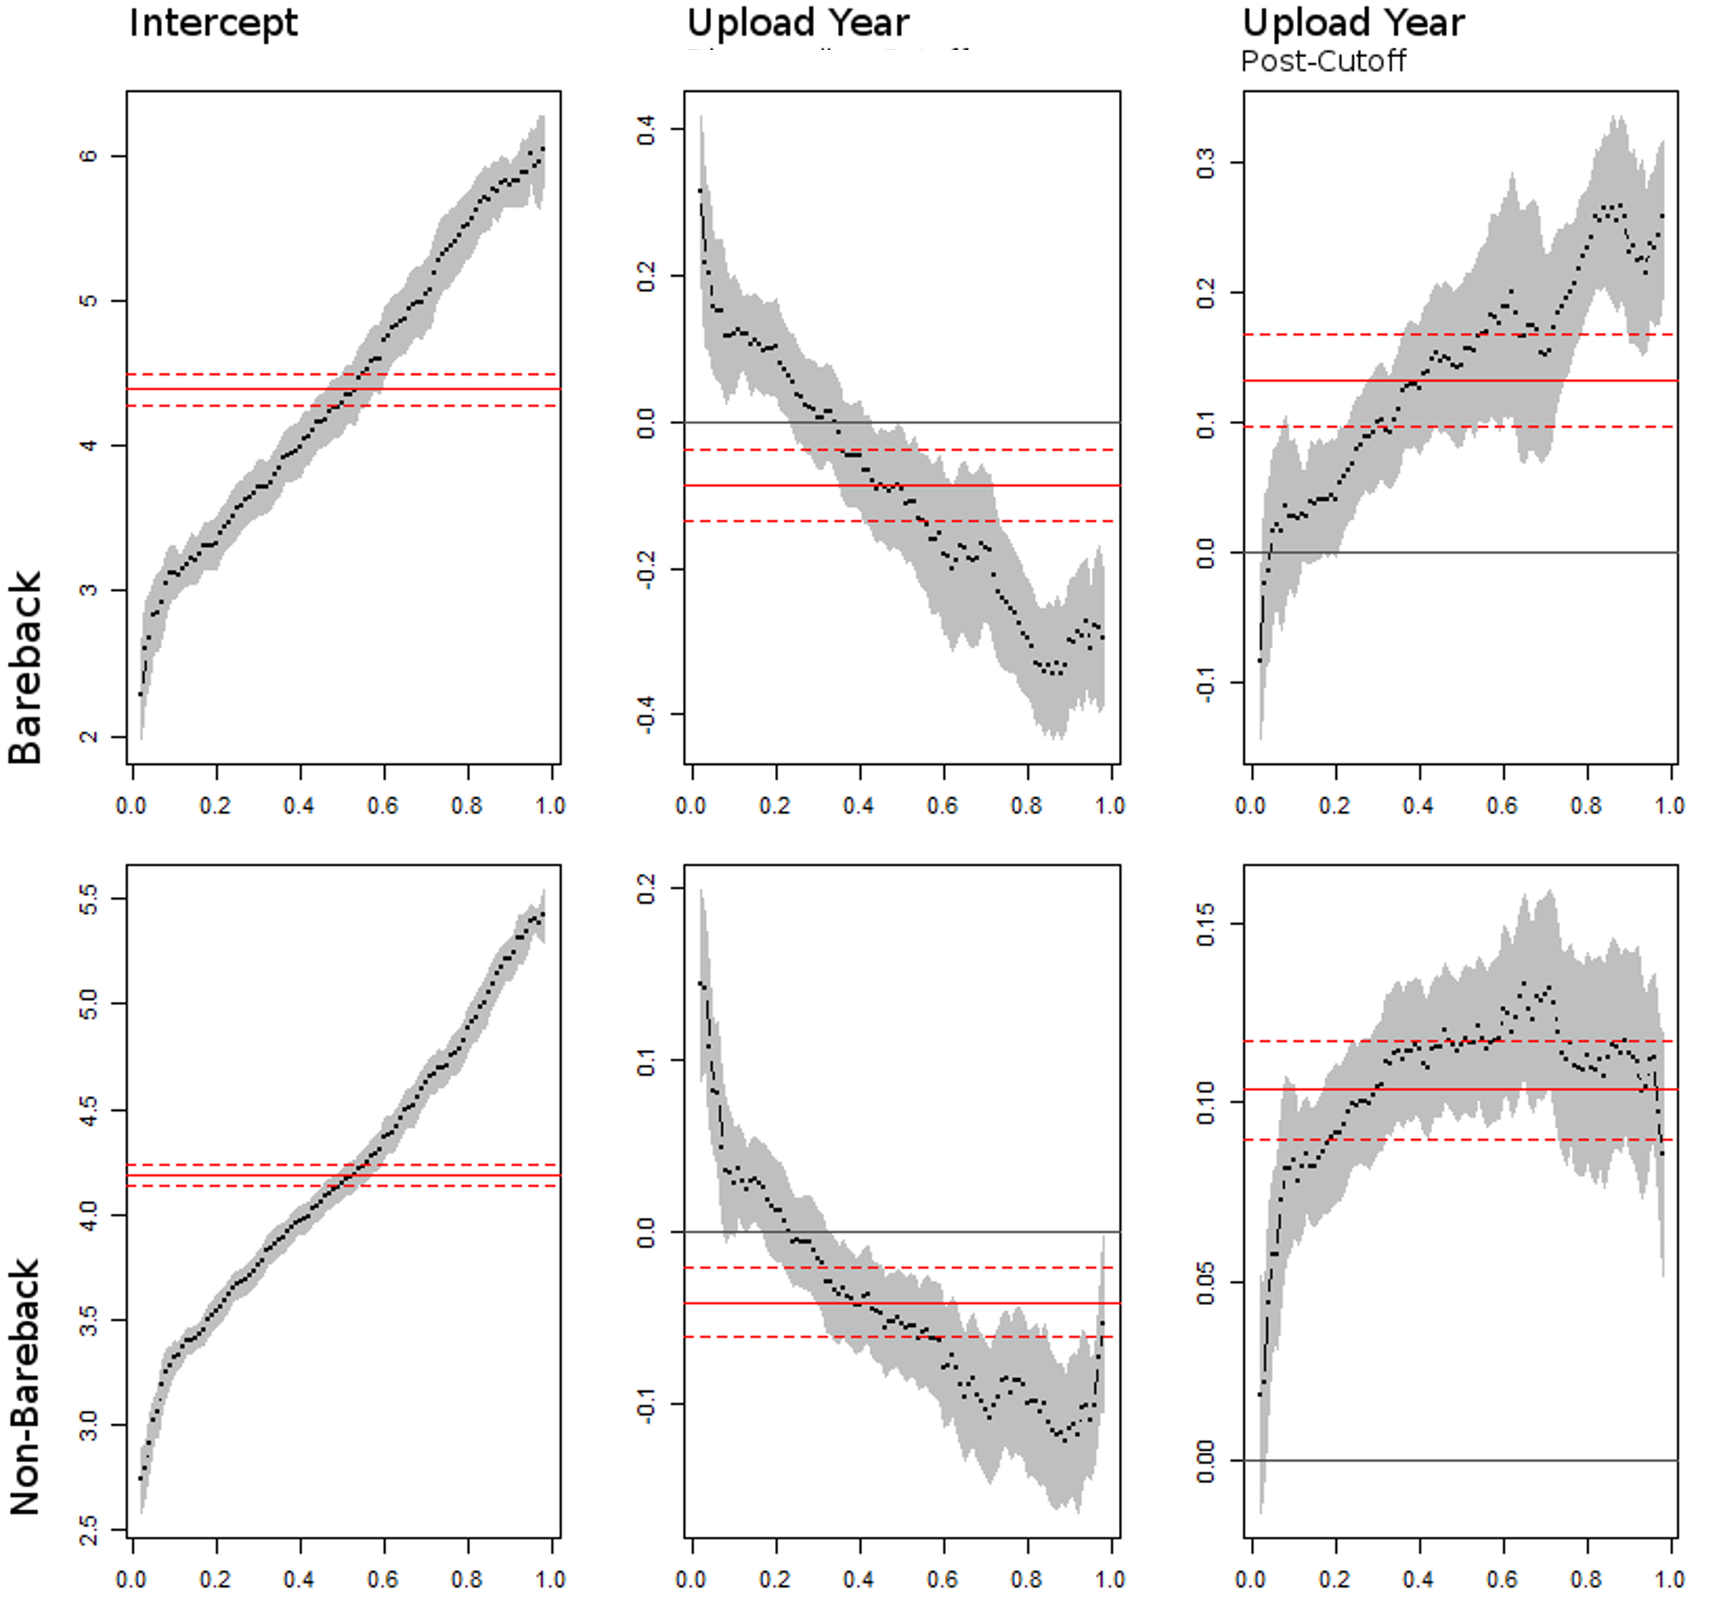
\includegraphics{./qrpfig.png}
\caption{\emph{Bareback videos enjoy more popularity across quantiles.}
Each panel of the quantile regression process for the log viewcount
model represents the vector-valued functions for each regression
coefficient among the subsample of videos differentiated by bareback
categorization. Y-axes are model coefficient values, X-axes are
\(\tau\). Grey bands indicate the 95\% confidence band estimates for
quantile values. Solid red lines are value means, with their associated
confidence interval depicted by dashed red lines. Note the differing
y-axes. As a general trend, videos categorized as bareback are more
popular than their non-bareback counterparts as measured by yearly log
quantile viewcount. A pronouced V-shape in the total slope coefficient
values is evident, indicative of both the utility of the splined upload
year term and potential residual bias in the sampling methodology.}
\end{figure}

An examination of the all of the distinct quantile regression solutions
for this model demonstrates a similar trend between bareback
categorization and upload year and their effect on view counts, though
the scale of these effects vary by categorization. Both bareback and
non-bareback videos have a similar median intercept view count
coefficient, though the range is larger for bareback videos (2 - 6
vs.~2.5 to 5.5). For both bareback and non-bareback videos, as \(\tau\)
increases the coefficient effect decreases, crossing the origin at
\$\tau \simeq \$ 0.25 for both videos. The strength of these changes are
most dramatic for bareback videos--at median view count, upload year
reduces log median view count by .1 for each year after 2010, which
non-bareback videos do not reach until the upper quartile, beginning at
\(\tau\) = 0.6 and hovering around this value for the higher quantiles.
The quantile process demonstrates two important temporal trends for
videos uploaded from 2010 to 2014: 1) the overall trend was a gradual
decline in log yearly quantile view count over time for both
categorizations of videos, and 2) the more popular videos categorized as
bareback (\(\tau \geq\) 0.5) are less likely to have been uploaded
before the cutoff determined by Truvada's approval.

The interaction term, a dummy variable for videos posted after the
cutoff multiplied by upload year, flips model coefficient slopes about
the origin for videos uploaded within the past 3 years. For bareback
categorized videos, however, the coefficient strength is as much as
doubled in the upper quantiles. Non-bareback videos plateau at the
60-70th percentile of videos by popularity, while the coefficient
strength continues to increase in a roughly linear fashion for bareback
videos until reaching an inflection point at \(\tau\) = 0.7. In
comparison with the magnitude of the opposing values of the uninteracted
upload year variable for equal \(\tau\) at quantiles greater than 0.6,
the net change in overall slope after the cutoff point is still in the
negative direction. For the majority of the quantile distribution,
however, net slope is in the positive direction, indicating a gradual
increase in popularity of videos over time across all but the most
popular bareback videos. A similar phenomenon is witnessed among
non-bareback videos for the same \(\tau\) range, though the magnitude of
the effect is not as great--bareback categorized videos remain more
popular overall. Despite this, inference from the quantile process
demonstrates an unsplined linear quantile model or linear regression on
the mean would have poorly captured trends in view counts across the
sample.

\begin{table}[]
\centering
\caption{Quintile Regression Model Coefficients. Coefficients demonstrate a pronounced "V"-shaped pattern to the regression slopes with vertex at the cutoff among both types of video content. Bareback videos experience a higher absolute value of views. Both year variables are in relation upload year since 2010. Intercept values should be interpreted as the log-transformed quintile view count for a video uploaded in 2010 by bareback categorization.}
\label{table1}
\begin{tabular}{@{}l|l|lll|lll@{}}
\toprule
\multicolumn{2}{l|}{}                                  & \multicolumn{3}{l|}{\textbf{Bareback}}                       & \multicolumn{3}{l}{\textbf{Not Bareback}}                  \\ \midrule
\textbf{Tau}                  & \textbf{Coefficient}   & \textbf{Value} & \textbf{SE} & \textbf{Pr(\textgreater|t|)} & \textbf{Value} & \textbf{SE} & \textbf{Pr(\textgreater|t|)} \\ \midrule
\multirow{3}{*}{\textbf{0.2}} & \textbf{Intercept}     & 3.325          & 0.104       & \textless 0.001              & 3.542          & 0.046       & \textless 0.001              \\
                              & \textbf{Year}          & 0.103          & 0.040       & \textless 0.001              & 0.012          & 0.018       & 0.50                         \\
                              & \textbf{Year : Cutoff} & 0.041          & 0.027       & 0.13                         & 0.091          & 0.012       & \textless 0.001              \\ \midrule
\multirow{3}{*}{\textbf{0.4}} & \textbf{Intercept}     & 3.981          & 0.115       & \textless 0.001              & 3.972          & 0.040       & \textless 0.001              \\
                              & \textbf{Year}          & -0.045         & 0.044       & 0.31                         & -0.042         & 0.017       & \textless 0.05               \\
                              & \textbf{Year : Cutoff} & 0.126          & 0.030       & \textless 0.001              & 0.115          & 0.012       & \textless 0.001              \\ \midrule
\multirow{3}{*}{\textbf{0.6}} & \textbf{Intercept}     & 4.718          & 0.147       & \textless 0.001              & 4.364          & 0.054       & \textless 0.001              \\
                              & \textbf{Year}          & -0.182         & 0.066       & \textless 0.01               & -0.079         & 0.021       & \textless 0.001              \\
                              & \textbf{Year : Cutoff} & 0.189          & 0.051       & \textless 0.001              & 0.126          & 0.014       & \textless 0.001              \\ \midrule
\multirow{3}{*}{\textbf{0.8}} & \textbf{Intercept}     & 5.514          & 0.142       & \textless 0.001              & 4.883          & 0.061       & \textless 0.001              \\
                              & \textbf{Year}          & -0.295         & 0.049       & \textless 0.001              & -0.100         & 0.025       & \textless 0.001              \\
                              & \textbf{Year : Cutoff} & 0.233          & 0.028       & \textless 0.001              & 0.113          & 0.018       & \textless 0.001              \\ \bottomrule
\end{tabular}
\end{table}

Table 1 lists quintile regression results with the proposed model fit.
The ``V''-shaped relationship between the model coefficients illustrated
above is most evident in the coefficients for upload year at the
\(\tau\) = 0.6 and 0.8 among both categorizations of videos, though the
magnitude of the intercept and slope coefficients among bareback videos
is greater. Significance of the upload year coefficient may be
instructive in delineating temporal trends in video popularity. Among
the lowest quintile, the interaction term \(\beta _{2, BB+}\) was not
significant (p = 0.13) for bareback videos, while for non-bareback
videos it was the uninteracted year term \(\beta _{1, BB-}\), evidence
that relatively unpopular bareback videos are more likely to have been
uploaded prior to the advent of PrEP while unpopular non-bareback videos
were more likely to have been uploaded after that time. This assessment
is reinforced by the relative strength of the counterpart year
coefficient (\(\beta _{1, BB+}\) = 0.103, p \textless{} 0.001;
\(\beta _{2, BB-}\) = 0.091, p \textless{} 0.001). The model positions
both types of videos roughly equivalently at \(\tau\) = 0.4, but from
there the model diverges by bareback categorization. Among bareback
videos, the upload year coefficients move from being roughly equivalent
in absolute value (\(\beta _{1, BB+}\) = -0.182, \(\beta _{2, BB+}\) =
0.189) at \(\tau\) = 0.6 to an overall reduction in popularity at the
highest quintile (\(\beta _{1, BB+} + \beta _{2, BB+}\) = -0.062 net
change in log-transformed yearly median view count) among videos
uploaded after the cutoff. Among non-bareback videos, the trend at these
quintiles is similar, though the overall change in popularity is greater
for videos posted after the cutoff.

The Khmaladze test is a test of the hypothesis that the linear model
specification is of the location shift or location-scale shift forms.
While it is clear from the quantile regression plots that we are not
dealing with a location-shift effect, as the coefficient curves would
fluctuate around a constant value, it also serves as a statistical test
of whether the distributions follow a location-scale shift effect. Based
on this analysis, and excluding the two most extreme quantiles in (0.05,
0.95), the joint test statistic for the model testing location-scale is
3.549 and 3.549 for the bareback categorized and not so categorized
videos, respectively. The asymptotic critical values at 1\% is 4.119
(Koenker and Xiao, 2001). The test statistic indicating the possibility
that the model specification is of the location-scale shift form is in
line with the insights from the visual examination of the quantile
process.

\subsubsection{Discussion}\label{discussion}

Data scraped from PornHub suggest an overall trend of higher view counts
among videos categorized as bareback than those that are not. Quantile
regression found distinctly higher quantile log view counts at all but
the earliest and most unpopular of video uploads.

The data also show a distinct shift in popularity of videos around the
cutoff point. Positioning the cutoff between the binned upload year
values of 2014 and 2015 was dictated by the CDC's approval of Truvada
having occurred in that time span; it was not driven by the data itself.
It is possible that the change in slope coefficient demonstrated by the
quantile regression model could be reflecting the impact of a trend
shift in viewing habits at an earlier time point. For example, the CDC
decision could have occurred after a growing popularity of unprotected
anal intercourse in PornHub consumer's preferences. Major advertisement
campaigns, a growing adoption and openness of PrEP among sexually active
gay men, and the use of ``hook-up apps'' could all have an effect on the
types of sexual content consumers may search for on pornographic
websites. The change in yearly proportion of bareback videos uploaded
after the cutoff, as well as their proportioon of total views,
strengthens the justification for the cutoff as assigned.

The ``V''-shaped pattern in the splined upload year terms with vertex at
the cutoff point could be an indication of residual measuring bias,
where the potential for increased views among older videos was not
properly accounted for, or an indication of competition among more
recently uploaded videos which may be more likely to appear together for
the consumer to choose from. It is also possible that the more popular
bareback videos were experiencing decline until secular trends around
the cutoff point reversed that trajectory--presumably, a major
announcement by the CDC, but other cultural phenomena could have taken
place. The proportion of yearly uploads that are bareback, and their
yearly view counts, suggest a trend change, however. The ``V'' pattern
in model slopes could also reflect the small subsample sizes of bareback
videos in the earliest upload year bins--if these happen to be quite
popular videos, it would throw off the regression analysis.

While this correlation in viewer preferences does not extend directly
into the actions of porn consumers, including safer sex practices and
PrEP adoption, it is a notable shift that could be indicative of these
and other phenomenon. Given what currently available research suggests
about the impact of viewing unprotected anal intercourse, growing
popularity of bareback videos has implications for public health
practitioners who work with men who have sex with men or in sexually
transmitted infection control. Considering also the potential
instructive role porn has in demonstrating sexuality to young MSM, who
also may not receive any competent or comprehensive sexuality education,
the import of bareback SEM could be magnified among younger viewers.

Moves toward widespread adoption of PrEP have been divisive, politically
and within gay culture. Concerns include the likelihood of PrEP being
used counter to the prescription, the potential for PrEP to undermine
existing safer sex policies and social mores, and the incredible cost of
the drug (as high as \$450 / month). Given the economic and social
capital that may be required to both receive and maintain adherence to a
PrEP prescription, and the relatively low bar required to have access to
online pornography, there are significant health equity concerns around
who may be most impacted by the viewership of unprotected anal
intercourse in gay SEM. According to the CDC, men who have sex with men
are at increased risk for sexually transmitted infections when compared
to women and exclusively heterosexual men (CDC, 2015). Researchers and
clinicians have noted an increase in sexually transmitted infections
among MSM--data from San Francisco show a steep climb in incident
gonorrhea and syphilis among both HIV-positive and HIV-negative gay men,
even while incident HIV cases continued to decline in what one
researcher termed a ``pretty fascinating epidemiological divide''
(Newman, 2016). While studies have demonstrated being HIV-positive and
using PrEP are both independently associated with a greater likelihood
of being diagnosed with an STI (Mayer et al., 2016), little research has
been undertaken demonstrating potentially changing cultural mores within
gay culture generally around the acceptability of unprotected anal
intercourse. More research is needed to examine the ways in which
non-clinical factors of gay male sociability and sexuality, including
pornography use, but also use of dating apps and interpersonal
communication, may also factor into the increasing trend of bacterial
sexually transmitted infections among men who have sex with men.

\paragraph{Limitations}\label{limitations}

The current study operates within several limitations, imposed by the
temporality of the study and the format of data storage from PornHub.
Due to PornHub's robots.txt, isolating viewership by country of consumer
was not possible. Their own published web traffic data by country allows
for a reasonable assumption that the broader trends found without
incorporating country code could reflect USA-specific viewing trends:
the US generates the most traffic and has the highest per capita page
views. The assumption was also made that MSM would seek out porn from
this gay porn section of the website. According to PornHub's own usage
statistics for 2016, \textasciitilde{}3\% of visitors from the US are
``gay visitors,'' a statistic that is commensurate with national surveys
on American's sexual orientation. This analysis was unable to control
for the identity of viewers, however, and 37\% of all gay male porn
views on PH are from women (PornHub, 2017). I was also unable to examine
videos behind PornHub's Premium service paywall. It is possible that
viewing habits and the videos themselves might differ between Premium
subscribers and users who only access content not behind a paywall.
According to CovenantEyes, a religiously-based anti-porn advocacy
organization modeled after consumer watchdogs, 9 out of 10 users access
free pornography (CovenantEyes, 2017).

For this analysis, I am relying on the host-supplied bareback
categorization in order to determine if a video contains sex between two
or more performers without use of condoms. Additionally, for the ``Solo
Male'' category, which is removed from the sample due to its inability
to capture the activity of interest, there is an added potential for
misclassification. Screening individual videos for unprotected anal
intercourse was outside of the scope of this project. Upload dates were
binned by year in the analysis, and only total view count amassed from
the unspecified upload dates to the time of scraping were able to be
examined. A finer resolution of upload date, or an ability to know the
viewing trends for each video since upload, would have refined the
analysis. Finally, the analysis was reliant on PornHub's organization of
videos into site indexes on category, which listed the 500 most recently
featured videos. There is no way to verify that the sample pooled from
such a filter represent fairly the video population as a whole, or the
selection criteria for videos to be recently featured.

\paragraph{Disclosure}\label{disclosure}

The author participated in the gay SEM industry from 2011 - 2016 and
wrote an op-ed against the Los Angeles County proposal mandating condom
use in SEM in 2012 (Cooper, 2012).

\begin{center}\rule{0.5\linewidth}{\linethickness}\end{center}

\subsubsection{References}\label{references}

Alexa. The Top 500 Sites on the Web. Alexa Top 500 Global Sites,
www.alexa.com/topsites. \url{https://www.alexa.com/topsites}

Braun-Courville, D. K., \& Rojas, M. (2009). Exposure to sexually
explicit web sites and adolescent sexual attitudes and behaviors.
Journal of Adolescent Health, 45(2), 156--162.

Center for Disease Control (2014). HIV PrEP Guidelines: New guidelines
recommend daily HIV prevention pill for those at substantial risk. May
14. Available online at
\url{https://www.cdc.gov/nchhstp/newsroom/2014/PrEP-Guidelines-Press-Release.html}.

Center for Disease Control (2015). STDs in Men Who Have Sex with Men.
2015 Seuxally Transmitted Diseaes Surveillance, Special Focus Profiles.
Available online at \url{https://www.cdc.gov/std/stats15/msm.htm}.

Cooper, D. Mismeasure B. The Huffington Post. Posted November 9, 2012.
\url{https://www.huffingtonpost.com/entry/mismeasure-b_b_2094384.html}

CovenantEyes (2017). Pornography Statistics: 2015 Report. Available
online at \url{http://www.covenanteyes.com/pornstats/}

Eaton, L. A., Cain, D. N., Pope, H., Garcia, J., \& Cherry, C. (2012).
The relationship between pornography use and sexual behaviors among
at-risk HIV-negative men who have sex with men. Sexual Health, 9(2),
166-170.

Grudzen, C. R., Elliot, M. N., Kerndt, P. R., Shuster, M. A., Brook, R.
H., \& Gelberg, L. (2009). Condom use and high-risk sexual acts in adult
films: A comparison of heterosexual and homosexual films. American
Journal of Public Health, 99(S1), S152-S156.

Koenker, R. (2017). quantreg: Quantile Regression. R package version
5.33. \url{https://CRAN.R-project.org/package=quantreg}

Koenker, R. and Xiao, Z. (2002). Inference on the quantile regression
process. Econometrica, 70:1583--1612.

Kubicek, K., Beyer, W. J., Weiss, G., Iverson, E., \& Kipke, M. D.
(2010). In the dark: Young men's stories of sexual initiation in the
absence of relevant sexual health information. Health Education \&
Behavior, 37(2), 243--263.

Los Angeles Times (2012). Porn industry declares war on new condom law.
November 8. Los Angeles Times. Retrieved from
\url{http://latimesblogs.latimes.com/lanow/2012/11/the-porn-industry-is-looking-for-ways-to-derail-a-voter-approved-ballot-measure-that-requires-actors-to-wear-condoms-during-f.html}

Mayer, K., Maloney, K., LEvine, K., King, D., Grasso, C., Krakower, D.,
and Boswell, S. HIV Infection and PrEP Use are Independently Associated
with Increasing Diagnoses of Bacterial Sexually Transmitted Infections
(BSTI) in Men Accessing Care at a Boston Community Health Center (CHC):
2005-2015. IDWeek 2016, Oral Abstract Session. Presented on October 29,
New Orleans.

Nelson, K. M., Simoni, J. M., Morrison, D. M., George, W. H., Leickly,
E., Lengua, L. L., \& Hawes, S. E. (2014). Sexually explicit online
media and sexual risk among men who have sex with men in the United
States. Archives of Sexual Behavior, 43, 833-843.

Newman, E. (2016). STDs Among Gay Men in a New Era of PrEP. BetaBlog.
June 16. Available online at
\url{http://betablog.org/stds-among-gay-men-new-era-prep/}.

Pornhub Insights (2017). Gay Porn Pride. June 22. Available online at
\url{https://www.pornhub.com/insights/gay-porn-pride}.

R Core Team (2017). R: A language and environment for statistical
computing. R Foundation for Statistical Computing, Vienna, Austria. URL
\url{https://www.R-project.org/}.

Rosser, B. R. S., Smolenski, D. J., Erickson, D. J., Iantaffi, A.,
Brady, S. S., Grey, J. A., \& Wilkerson, J. M. (2013). The effects of
gay sexually explicit media on the HIV risk behavior of men who have sex
with men. AIDS and Behavior, 17(4), 1488--1498.
\url{doi:10.1007/s10461-013-0454-8}

Schrimshaw EW, Antebi-Gruszka N, Downing MJ Jr. Viewing of
Internet-Based Sexually Explicit Media as a Risk Factor for Condomless
Anal Sex among Men Who Have Sex with Men in Four U.S. Cities. PLoS One.
2016 Apr 27;11(4):e0154439.

Stein, D., Silvera, R., Hagerty, R., \& Marmor, M. (2012). Viewing
pornography depicting unprotected anal intercourse: Are there
implications for HIV prevention among men who have sex with men.
Archives of Sexual Behavior, 41(2), 411-419.

Træen, B., Hald, G., Noor, S., Iantaffi, A., Grey, J. A., \& Rosser, B.
R. S. (2014). The relationship between use of sexually explicit media
and sexual risk behavior in men who have sex with men: Exploring the
mediating effects of sexual self-esteem and condom use self-efficacy.
International Journal of Sexual Health, 26, 13--24.

Wallace, B. (2011). The Geek Kings of Smut. New York Times Magazine. Feb
7. Online at
\url{https://web.archive.org/web/20141010205213/http://nymag.com/news/features/70985/index4.html}.

Wickham, H. (2016). rvest: Easily Harvest (Scrape) Web Pages. R package
version 0.3.2. \url{https://CRAN.R-project.org/package=rvest}

Williams, L. (1992). `Pornographies On/Scene, or Diff'rent Strokes for
Diff'rent Folks.' In Sex Exposed: Sexuality and the Pornography Debate,
edited by Lynne Segal and Mary McIntosh, 233-265. London: Virago.

Wilkerson, J. M., Inataffi, A., Smolenski, D. J., Brady, S. S., Horvath,
K. J., Grey, J. A., \& Rosser, B. R. S. (2012). The SEM risk behavior
(SRB) model: A new conceptual model of how pornography influences the
sexual intentions and HIV risk behavior of MSM. Sexual and Relationship
Therapy, 27(3), 217-230.


\end{document}
